\chapter{Environment}
\label{chapter:environment}

\section{Related Web Technology}

Describe HTML5, JS and other related technology, because these are really the things that restrict the implementation.

Visualizations need to be implemented using web technology, because it is crucial for distributability and discoverability that the system works in web browsers... \fixme{continue...}

\section{Current Map Visualizations} % TODO come up with a better title

Describe the map visualizations that sparked the interest for this kind of research. FindBooze, Peruskartta and Ottoapp. Also, reason why it is unnecessarily laborious to write map visualizations every time from scratch.

\section{Instructions}

A problem instance is rarely totally independent of its environment.
Most often you need to describe the environment you work in, what
limits there are and so on. This is a good place to do that. First we
tell you about the LaTeX working environments and then is an example
from an thesis written some years ago.

\section{\LaTeX\ Graphics}

When you use \texttt{pdflatex} to render your thesis, you can include PDF images
directly, as shown by Figure~\ref{fig:indica_model} below.

\begin{figure}[ht]
  \begin{center}
    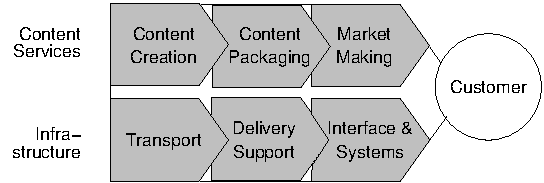
\includegraphics[width=\textwidth]{images/indica_model.pdf}
    \caption{The INDICA two-layered value chain model.}
    \label{fig:indica_model}
  \end{center}
\end{figure}

You can also include JPEG or PNG files, as shown by Figure~\ref{fig:eeyore}.

\begin{figure}[ht]
  \begin{center}
    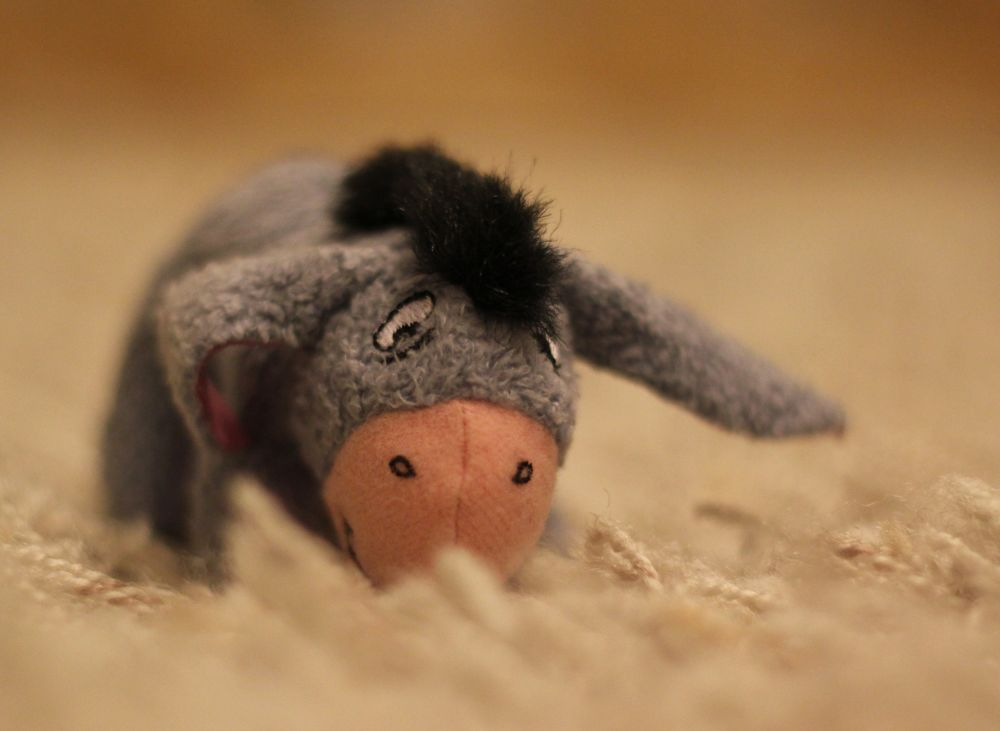
\includegraphics[width=9cm]{images/ihaa.jpg}
    \caption{Eeyore, or Ihaa, a very sad donkey.}
    \label{fig:eeyore}
  \end{center}
\end{figure}

You can create PDF files out of practically anything. 
In Windows, you can download PrimoPDF or CutePDF (or some such) and install a
printing driver so that you can print directly to PDF files from any
application. There are also tools that allow you to upload documents in common
file formats and convert them to the PDF format.
If you have PS or EPS files, you can use the tools \texttt{ps2pdf} or
\texttt{epspdf} to convert your PS and EPS files to PDF\@.

% Comment: If your sentence ends in a capital letter, like here, you should
% write \@ before the period; otherwise LaTeX will assume that this is not
% really an end of the sentence and will not put a large enough space after the
% period. That is, LaTeX assumes that you are (for example), enumerating using
% capital roman numerals, like I. do something, II. do something else. In this
% case, the periods do not end the sentence.

% Similarly, if you do need a normal space after a period (instead of
% the longer sentence separator), use \  (backslash and space) after the
% period. Like so: a.\ first item, b.\ second item.

Furthermore, most newer editor programs allow you to save directly to the PDF
format. For vector editing, you could try Inkscape, which is a new open source
WYSIWYG vector editor that allows you to save directly to PDF\@. 
For graphs, either export/print your graphs from OpenOffice Calc/Microsoft
Excel to PDF format, and then add them; or use \texttt{gnuplot}, which can
create PDF files directly (at least the new versions can).
The terminal type is \emph{pdf}, so the first line of your plot file should be
something like \texttt{set term pdf \ldots}.

To get the most professional-looking graphics, you can encode them using the
TikZ package (TikZ is a frontend for the PGF graphics formatting system).
You can create practically any kind of technical images with TikZ, but it has a
rather steep learning curve. Locate the manual (\texttt{pgfmanual.pdf}) from
your \LaTeX\ distribution and check it out. An example of TikZ-generated
graphics is shown in Figure~\ref{fig:page-merge}.

\begin{figure}[ht]
  \begin{center}
    \newcommand*{\actver}{\smash{\ensuremath{v_{\text{\textit{active}}}}}}

\tikzstyle{lbl}=[font=\scriptsize,midway,sloped]
\tikzstyle{opendash}=[densely dotted,thick] 
\tikzstyle{opendeco}=[decoration={zigzag,amplitude=0.1em,segment length=0.6em}]
\tikzstyle{actverline}=[dashed]
\tikzstyle{entryline}=[densely dotted]
\tikzstyle{area}=[ellipse,draw,dashed]
\tikzstyle{liveentry}=[entryline,postaction={%
  decorate,%
  decoration={%
    markings,%
    mark=at position .5pt with{\arrowreversed[line width=.35pt]{|}};,
    mark=at position 1 with{%
      \arrow[line width=.8pt]{stealth}};%
  }%
}]
\tikzstyle{deadentry}=[entryline,postaction={%
  decorate,%
  decoration={%
    markings,%
    mark=at position .5pt with{\arrowreversed[line width=.35pt]{|}};,
    mark=at position 1 with{%
      \arrow[line width=.8pt]{stealth}};%
%      \arrow[line width=.35pt,black,fill=white]{*}};% 
  }%
}]
\tikzstyle{pageborder}=[thick]
\tikzstyle{pagename}=[anchor=center,text=black!50,font=\huge]
\newlength{\spexx}
\setlength{\spexx}{1.2cm}
\newlength{\spexy}
\setlength{\spexy}{.5cm}

\subfigure[Before]{
\begin{tikzpicture}[x=\spexx,y=\spexy,%
  every pin edge/.style={draw,dotted},%
  pin distance=.5\spexx]
  \small
  \coordinate (lo) at (0,-5);
  \coordinate (o) at (0,0);
  \coordinate (hi) at (0,7);
  \coordinate (loact) at (3,-5);
  \coordinate (oact) at (3,0);
  \coordinate (hiact) at (3,7);
  \coordinate (loinf) at (4,-5);
  \coordinate (oinf) at (4,0);
  \coordinate (hiinf) at (4,7);
  
  \draw[->] (lo) -- node[below,lbl] {Versions} ($(loinf) + (1em,0)$);
  \draw[->] (lo) -- node[above,lbl] {Keys} ($(hi) + (0,1em)$);

  \draw[pageborder] (lo) -- (o) -- (hi);
  \draw[pageborder] (lo) -- (loinf);
  \draw[pageborder] (hi) -- (hiinf);
  \draw[pageborder] (o) -- (oinf);

  \draw[opendash] decorate [opendeco] { (loinf) -- (oinf) };
  \draw[opendash] decorate [opendeco] { (oinf) -- (hiinf) };

  \node[pagename] at (2,3.5) {$p$};
  \node[pagename] at (2,-2.5) {$s$};

  \draw[actverline] ($(loact) + (0,-1em)$) node[below=.4em] {\actver} --
    ($(hiact) + (0,1em)$);

  % Page p contents
  \draw[deadentry] (0,6) -- (1,6);
  \draw[deadentry] (1,6) -- (2,6);
  \draw[deadentry] (2,6) -- (3,6);
  \draw[liveentry] (0,5) -- (4,5);
  \draw[deadentry] (0,4) -- (2,4);
  \draw[deadentry] (1,3) -- (3,3);
  \draw[deadentry] (0,2) -- (1,2);
  \draw[deadentry] (2,2) -- (3,2);
  \draw[deadentry] (0,1) -- (2,1);
  \draw[deadentry] (2,1) -- (3,1);

  % Page s contents
  \draw[liveentry] (0,-1) -- (4,-1);
  \draw[deadentry] (0,-2) -- (2,-2);
  \draw[deadentry] (0,-3) -- (3,-3);
  \draw[liveentry] (3,-4) -- (4,-4);

  \node[area,minimum width=4.5\spexx,minimum height=.6\spexy,pin=178:{$1$}]
    at (2,5) {};
  \node[area,minimum width=4.5\spexx,minimum height=.6\spexy,pin=182:{$2$}]
    at (2,-1) {};
  \node[area,minimum width=1.5\spexx,minimum height=.6\spexy,pin=330:{$3$}]
    at (3.5,-4) {};

\end{tikzpicture}}
\subfigure[After]{
\begin{tikzpicture}[x=\spexx,y=\spexy,%
  every pin edge/.style={draw,dotted},%
  pin distance=.5\spexx]
  \small
  \coordinate (lo) at (0,-5);
  \coordinate (o) at (0,0);
  \coordinate (hi) at (0,7);
  \coordinate (loact) at (3,-5);
  \coordinate (oact) at (3,0);
  \coordinate (hiact) at (3,7);
  \coordinate (loinf) at (4,-5);
  \coordinate (oinf) at (4,0);
  \coordinate (hiinf) at (4,7);

  \draw[->] (lo) -- node[lbl,below] {Versions} ($(loinf) + (1em,0)$);
  \draw[->] (lo) -- node[lbl,above] {Keys} ($(hi) + (0,1em)$);

  \draw[pageborder] (lo) -- (o) -- (hi);
  \draw[pageborder] (lo) -- (loinf);
  \draw[pageborder] (hi) -- (hiinf);
  \draw[pageborder] (o) -- (oact);

  \draw[opendash] decorate [opendeco] { (loinf) -- (oinf) };
  \draw[opendash] decorate [opendeco] { (oinf) -- (hiinf) };

  \node[pagename] at (1.5,3.5) {$p$};
  \node[pagename] at (1.5,-2.5) {$s$};
  \node[pagename] at (3.5,1) {$p'$};

  \draw[actverline] ($(loact) + (0,-1em)$) node[below=.4em] {\actver} -- (loact);
  \draw[pageborder] (loact) -- (hiact);
  \draw[actverline] (hiact) -- ($(hiact) + (0,1em)$);

  % Page p contents
  \draw[deadentry] (0,6) -- (1,6);
  \draw[deadentry] (1,6) -- (2,6);
  \draw[deadentry] (2,6) -- (3,6);
  \draw[deadentry] (0,5) -- (3,5);
  \draw[deadentry] (0,4) -- (2,4);
  \draw[deadentry] (1,3) -- (3,3);
  \draw[deadentry] (0,2) -- (1,2);
  \draw[deadentry] (2,2) -- (3,2);
  \draw[deadentry] (0,1) -- (2,1);
  \draw[deadentry] (2,1) -- (3,1);

  % Page s contents
  \draw[deadentry] (0,-1) -- (3,-1);
  \draw[deadentry] (0,-2) -- (2,-2);
  \draw[deadentry] (0,-3) -- (3,-3);

  % Page p' contents
  \draw[liveentry] (3,5) -- (4,5);
  \draw[liveentry] (3,-1) -- (4,-1);
  \draw[liveentry] (3,-4) -- (4,-4);

  \node[area,minimum width=1.5\spexx,minimum height=.6\spexy,pin=10:{$1$}]
    at (3.5,5) {};
  \node[area,minimum width=1.5\spexx,minimum height=.6\spexy,pin=3:{$2$}]
    at (3.5,-1) {};
  \node[area,minimum width=1.5\spexx,minimum height=.6\spexy,pin=330:{$3$}]
    at (3.5,-4) {};
\end{tikzpicture}}

    \caption{Example of a multiversion database page merge. This figure has
    been taken from the PhD thesis of Haapasalo~\citep{HaapasaloThesis}.}
    \label{fig:page-merge}
  \end{center}
\end{figure}

Another example of graphics created with TikZ is shown in
Figure~\ref{fig:tikz-examples}. 
These show how graphs can be drawn and labeled. 
You can consult the example images and the PGF manual for more examples of what
kinds figures you can draw with TikZ. 

% These definitions are only used in the example images; you will not 
% need them for your thesis...
\newlength{\graphdotsize}
\setlength{\graphdotsize}{1.7pt}
\newlength{\graphgridsize}
\setlength{\graphgridsize}{1.2em}
\begin{figure}[ht]
\begin{center}
\subfigure[Examples of obstruction graphs for the Ferry Problem]{
  \newlength{\oggs}
\setlength{\oggs}{1.2\graphgridsize}
\begin{tikzpicture}[x=\oggs,y=\oggs,every pin edge/.style={draw,dotted},pin distance=0.5\oggs,area/.style={ellipse,draw,dashed}] 

% The graph (0,0,5,0)
% o = origo
\coordinate (o) at (0,0);
\coordinate[left=1 of o,pin=100:$q_1$] (q1);
\coordinate[right=1 of o,pin=80:$q_2$] (q2);
\fill[black] (q1) circle (\graphdotsize);
\fill[black] (q2) circle (\graphdotsize);
\foreach \d in {-2, -1, ..., 2} {
  \coordinate (tmp) at ($(o) + (0,\d)$);
  \draw (q1) -- (tmp);
  \draw (q2) -- (tmp);
  \fill[black] (tmp) circle (\graphdotsize);
}
\node[area,minimum height=5.3\oggs,minimum width=0.8\oggs,pin=94:$X_3$] at (o) {};  

% The graph (1,0,3,0)
\coordinate[right=5 of o] (o);
\coordinate[left=1 of o,pin=260:$q_1$] (q1);
\coordinate[left=2 of o] (q1v);
\coordinate[right=1 of o,pin=280:$q_2$] (q2);
\fill[black] (q1) circle (\graphdotsize);
\fill[black] (q2) circle (\graphdotsize);
\fill[black] (q1v) circle (\graphdotsize);
\draw (q1) -- (q1v);
\foreach \d in {-1, 0, 1} {
  \coordinate (tmp) at ($(o) + (0,\d)$);
  \draw (q1) -- (tmp);
  \draw (q2) -- (tmp);
  \fill[black] (tmp) circle (\graphdotsize);
}
\node[area,minimum height=3.3\oggs,minimum width=0.8\oggs,pin=266:$X_3$] at (o) {};  
\node[area,minimum height=0.8\oggs,minimum width=0.8\oggs,pin=260:$X_1$] at (q1v) {};  


% The graph (0,1,3,0)
\coordinate[right=4 of o] (o);
\coordinate[left=1 of o,pin=100:$q_1$] (q1);
\coordinate[right=1 of o,pin=80:$q_2$] (q2);
\coordinate[right=2 of o] (q2v);
\fill[black] (q1) circle (\graphdotsize);
\fill[black] (q2) circle (\graphdotsize);
\fill[black] (q2v) circle (\graphdotsize);
\draw (q2) -- (q2v);
\foreach \d in {-1, 0, 1} {
  \coordinate (tmp) at ($(o) + (0,\d)$);
  \draw (q1) -- (tmp);
  \draw (q2) -- (tmp);
  \fill[black] (tmp) circle (\graphdotsize);
}
\node[area,minimum height=3.3\oggs,minimum width=0.8\oggs,pin=94:$X_3$] at (o) {};  
\node[area,minimum height=0.8\oggs,minimum width=0.8\oggs,pin=80:$X_2$] at (q2v) {};  

% The graph (0,0,3,1)
\coordinate[right=5 of o] (o);
\coordinate[left=1 of o,pin=260:$q_1$] (q1);
\coordinate[right=1 of o,pin=290:$q_2$] (q2);
\fill[black] (q1) circle (\graphdotsize);
\fill[black] (q2) circle (\graphdotsize);
\draw (q1) -- (q2);
\foreach \d in {-1, 1, 2} {
  \coordinate (tmp) at ($(o) + (0,\d)$);
  \draw (q1) -- (tmp);
  \draw (q2) -- (tmp);
  \fill[black] (tmp) circle (\graphdotsize);
}
\node[area,minimum height=4.3\oggs,minimum width=0.8\oggs,pin=266:$X_3$] at ($(o) + (0,0.5)$) {};  

\end{tikzpicture}

}
\subfigure[Examples of star graphs]{
  \begin{tikzpicture}[x=\graphgridsize,y=\graphgridsize] 

\coordinate (o) at (0,0);
\fill[black] (o) circle (\graphdotsize);
\foreach \d in {0, 90, ..., 270} {
  \coordinate (tmp) at ($(o) + (\d:1.5)$);
  \draw (o) -- (tmp);
  \fill[black] (tmp) circle (\graphdotsize);
}

\coordinate[right=4 of o] (o);
\coordinate (o1) at ($(o) + (0:0.3)$);
\coordinate (o2) at ($(o) + (180:0.3)$);
\fill[black] (o1) circle (\graphdotsize);
\fill[black] (o2) circle (\graphdotsize);
\draw (o1) -- (o2);
\foreach \d in {45, 135, 270} {
  \coordinate (tmp\d) at ($(o) + (\d:1.5)$);
  \draw (o2) -- (tmp\d);
  \fill[black] (tmp\d) circle (\graphdotsize);
}
\draw (o1) -- (tmp45);


\coordinate[right=4 of o] (o);
\coordinate (o1) at ($(o) + (0:0.3)$);
\coordinate (o2) at ($(o) + (180:0.3)$);
\fill[black] (o1) circle (\graphdotsize);
\fill[black] (o2) circle (\graphdotsize);
\draw (o1) -- (o2);
\foreach \d in {45, 135, 270} {
  \coordinate (tmp\d) at ($(o) + (\d:1.5)$);
  \draw (o2) -- (tmp\d);
  \fill[black] (tmp\d) circle (\graphdotsize);
}
\draw (o1) -- (tmp45);
\draw (o1) -- (tmp135);


\coordinate[right=4 of o] (o);
\coordinate (o1) at ($(o) + (0:0.3)$);
\coordinate (o2) at ($(o) + (180:0.3)$);
\fill[black] (o1) circle (\graphdotsize);
\fill[black] (o2) circle (\graphdotsize);
\draw (o1) -- (o2);
\foreach \d in {45, 135, 270} {
  \coordinate (tmp\d) at ($(o) + (\d:1.5)$);
  \draw (o1) -- (tmp\d);
  \draw (o2) -- (tmp\d);
  \fill[black] (tmp\d) circle (\graphdotsize);
}


\coordinate[right=3.5 of o] (o);
\coordinate (o1) at ($(o) + (90:0.3)$);
\coordinate (o2) at ($(o) + (210:0.5)$);
\coordinate (o3) at ($(o) + (330:0.5)$);
\fill[black] (o1) circle (\graphdotsize);
\fill[black] (o2) circle (\graphdotsize);
\fill[black] (o3) circle (\graphdotsize);
\draw (o1) -- (o2);
\draw (o1) -- (o3);
\draw (o2) -- (o3);
\foreach \d in {90, 270} {
  \coordinate (tmp\d) at ($(o) + (\d:1.5)$);
  \draw (o2) -- (tmp\d);
  \draw (o3) -- (tmp\d);
  \fill[black] (tmp\d) circle (\graphdotsize);
}
\draw (o1) -- (tmp90);


\coordinate[right=3 of o] (o);
\coordinate (o1) at ($(o) + (90:0.3)$);
\coordinate (o2) at ($(o) + (210:0.5)$);
\coordinate (o3) at ($(o) + (330:0.5)$);
\fill[black] (o1) circle (\graphdotsize);
\fill[black] (o2) circle (\graphdotsize);
\fill[black] (o3) circle (\graphdotsize);
\draw (o1) -- (o2);
\draw (o1) -- (o3);
\draw (o2) -- (o3);
\foreach \d in {90, 270} {
  \coordinate (tmp\d) at ($(o) + (\d:1.5)$);
  \draw (o2) -- (tmp\d);
  \draw (o3) -- (tmp\d);
  \fill[black] (tmp\d) circle (\graphdotsize);
}
\draw (o1) -- (tmp90);
\draw (o1) -- (tmp270);



\coordinate[right=3.5 of o] (o);
\coordinate (o1) at ($(o) + (18:1.3)$);
\coordinate (o2) at ($(o) + (90:1.3)$);
\coordinate (o3) at ($(o) + (162:1.3)$);
\coordinate (o4) at ($(o) + (234:1.3)$);
\coordinate (o5) at ($(o) + (306:1.3)$);
\foreach \d in {1, 2, ..., 5} {
  \fill[black] (o\d) circle (\graphdotsize);
}
\draw (o1) -- (o2);
\draw (o1) -- (o3);
\draw (o1) -- (o4);
\draw (o1) -- (o5);
\draw (o2) -- (o3);
\draw (o2) -- (o4);
\draw (o2) -- (o5);
\draw (o3) -- (o4);
\draw (o3) -- (o5);
\draw (o4) -- (o5);

\end{tikzpicture}

}
\caption{Examples of graphs draw with TikZ. These figures have been taken from a
course report for the graph theory course~\citep{FerryProblem}.}
\label{fig:tikz-examples}
\end{center}
\end{figure}

